\documentclass[12pt]{article}
\usepackage{lingmacros}
\usepackage{tree-dvips}
\usepackage{amsmath}
\usepackage{IEEEtrantools}
\usepackage{amssymb}
\usepackage{graphicx}
\usepackage{float}
\usepackage{sectsty}
\usepackage{xstring}
\usepackage{xparse}
\graphicspath{ {./images/} }

\iffalse
	\sectionfont{\fontsize{16}{15}\selectfont}
\fi

% *** Magic Commands! *** %

	% call empty: \coherent[]{S}
	% call with index: \coherent[0]{S+l}
	\NewDocumentCommand\coherent{om}{%
		\IfNoValueTF{#1}
		{$|#2\rangle$}
		{$|#2_#1\rangle$}%
	}

	\newcommand{\logH}[1]{#1log{\left[\frac{1}{#1}\right]}}

	\newcommand{\lambdaWave}{\overline{\lambda}}

	\newcommand{\lambdaSwitch}[1]{%
		\IfEqCase{#1}{%
			{0}{\lambda_0=|S_0+l|^2}%
			{1}{\lambda_1=|S_1+l|^2}%
			{i}{\lambda_i=|S_i+l|^2}%
			{~}{\widetilde{\lambda}=\pi_{0}\sqrt{\lambda_{0}}+\pi_{1}\sqrt{\lambda_{1}}}%
			{-}{\lambdaWave=\pi_{0}\lambda_{0}+\pi_{1}\lambda_{1}}%
			% you can add more cases here as desired
		}[\PackageError{tree}{Undefined option to tree: #1}{}]%
	}%

	\newcommand{\piSwitch}[1]{%
		\IfEqCase{#1}{%
			{0}{$\pi_{0} = \frac{g}{g+1}$}%
			{1}{$\pi_{1} = \frac{1}{g+1}$}%
			% you can add more cases here as desired
		}[\PackageError{tree}{Undefined option to tree: #1}{}]%
	}%

	\newcommand{\g}{$g = \pi_{0}/\pi_{1}$}
	\newcommand{\lStar}{\frac{S_{0}\pi_{0} - S_{1}\pi_{1}}{\pi_{1}-\pi_{0}}}

	\newcommand{\piG}[1]{%
		\IfEqCase{#1}{%
			{0}{$\pi_{0} = \frac{g}{g+1}$}%
			{1}{$\pi_{1} = \frac{1}{g+1}$}%
			% you can add more cases here as desired
		}[\PackageError{tree}{Undefined option to tree: #1}{}]%
	}%

% *********************** %


\begin{document}

	\begin{equation}
		\left( \left( \right) \right) \amalg\rightthreetimes\\
		bla
	\end{equation}	

	\begin{center}
		\section*{Signal detection over an optical channel}
	
	\end{center}
	\vspace{0.5cm}

	\piSwitch{0},\quad\g,\quad $\lambdaSwitch{1}$,\quad\piG{0},\quad$\lStar$\\\\\\
	 
	Given an optical channel, a signal on that channel can be described as a coherent state denoted by \coherent{S} where  $S\in\mathbb{C}$\\

	Considering a Noise free environment, in order to detect a signal in this type of channel, 
	we use a photon counter receiver. Such a receiver is a direct detection receiver which detects 
	the intensity of the optical and generates a Poisson process, where the rate of the process holds $\lambda = |S|^2$ .\\
	
	Suppose we have two coherent state signals denoted by \coherent[0]{S}, \coherent[1]{S} and we would like to distinguish between the two 
	binary hypotheses with the corresponding priori probabilities $\pi_0, \pi_1$ respectively under hypotheses $H=0,1$, 
	while holding some transmission cost constraint.\\
	
	One approach was given by \textbf{Kennedy} who proposed adding a constant additional coherent state signal \coherent{l}
	before feeding the signal’s input to the receiver. Doing so generates a coherent state \coherent{S+l} which 
	the receiver in turn outputs a Poisson process with rate $\lambdaSwitch{i}$.\\

	An additional approach was given by \textbf{Dolinar} who suggested as continuation to Kennedy’s design to replace the constant 
	signal with a controlled signal \coherent{l(t)} which is chosen adaptively based on the photon arrivals up to that moment, 
	in order to achieve more certainty in the hypothesis choice with time.\\

	The core concept of Dolinar’s updated design includes a recursive method in which the posterior probabilities of 
	the two possible hypotheses denoted by $\pi_1(t), \pi_2(t)$ are updated after each step of time $\Delta$ to yield 
	$\pi_1(t+\Delta), \pi_2(t+\Delta)$.\\
	
	At this point, by making $\Delta$ arbitrarily small we can expect the current Poisson process to return:
	\begin{equation*}
		Poisson(\lambda) = \left\{ \,
		\begin{IEEEeqnarraybox}[][c]{l?s}
			\IEEEstrut
				0 & w.p. $(1-\lambda_i\Delta)$\\
				1 & w.p. $(\lambda_i\Delta)$
			\IEEEstrut
		\end{IEEEeqnarraybox}
		\right.
		\label{eq:example_left_right1}
	\end{equation*}\\

	Which can be thought of as the following binary channel (Figure \ref{fig:channel}):\\

	\pagebreak[2]
	\begin{figure}[H]
		\centering
		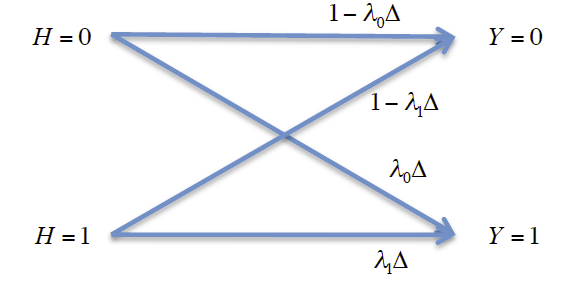
\includegraphics[width=8cm]{channel.png}
		\caption{Equivalent binary channel over time $\Delta$}
		\label{fig:channel}
	\end{figure}

	Since we obtained an approximation of a binary channel we may now ask how should $\l(t)$ be decided in 
	other to maximize the mutual information of the binary channel.\\
	
	The Entropy can be calculated as follows:
	\begin{IEEEeqnarray*}{rCl}
		\IEEEeqnarraymulticol{3}{l}
		{
			H(Y)=H_{b}[\Delta(\pi_{0}\lambda_{0} + \pi_{1}\lambda_{1})]
		}\\*
		H(Y|X)=\pi_{0}H_{b}(\Delta\lambda_{1}) + \pi_{1}H_{b}(\Delta\lambda_{1})
	\end{IEEEeqnarray*}

	Which gives us the mutual information of the channel:\\

	\begin{IEEEeqnarray*}{rCl}
		\IEEEeqnarraymulticol{3}{l}
		{
			I(X;Y)=H(Y)-H(Y|X)
		}
		\nonumber\\*=H_{b}[\Delta(\pi_{0}\lambda_{0} + \pi_{1}\lambda_{1})]
		\nonumber\\*\qquad\qquad-\left[\pi_{0}H_{b}(\Delta\lambda_{1}) + \pi_{1}H_{b}(\Delta\lambda_{1})\right]
		\label{eq:dont_use_multline}
	\end{IEEEeqnarray*}

	\pagebreak[4]

	Since we want to maximize the mutual information, we shall compare its derivative to zero:
	
	\begin{IEEEeqnarray*}{rCl}
		\IEEEeqnarraymulticol{3}{l}
		{
			\frac{dI(X;Y)}{dl} = 
			\log_{2}\left[\frac
				{1-\Delta[\pi_{0}\lambda_{0}+\pi_{1}\lambda_{1}]}
				{\Delta[\pi_{0}\lambda_{0}+\pi_{1}\lambda_{1}]}\right]
			2\Delta(\pi_{0}\sqrt{\lambda_{0}}+\pi_{1}\sqrt{\lambda_{1}})
		}\\*
		\qquad\qquad\qquad-\log_{2}\left[\frac{1-\lambda_{0}\Delta}{\lambda_{0}\Delta}\right]2\Delta\pi_{0}\sqrt{\lambda_{0}}\\*
		\qquad\qquad\qquad-\log_{2}\left[\frac{1-\lambda_{1}\Delta}{\lambda_{1}\Delta}\right]2\Delta\pi_{1}\sqrt{\lambda_{1}}\\*
		\qquad\qquad\qquad=0
	\end{IEEEeqnarray*}

	\begin{IEEEeqnarray*}{rCl}
		\IEEEeqnarraymulticol{3}{l}
		{
			\frac{dI(X;Y)}{dl} = 
			\log_{2}\left[\frac
				{1-\Delta[\pi_{0}\lambda_{0}+\pi_{1}\lambda_{1}]}
				{\Delta[\pi_{0}\lambda_{0}+\pi_{1}\lambda_{1}]}\right]
			2\Delta(\pi_{0}\sqrt{\lambda_{0}}+\pi_{1}\sqrt{\lambda_{1}})
		}\\*
		\qquad\qquad\qquad-2\Delta\left[\log_{2}\left(\frac{1-\lambda_{0}\Delta}{\lambda_{0}\Delta}\right)\pi_{0}\sqrt{\lambda_{0}}
			+\log_{2}\left(\frac{1-\lambda_{1}\Delta}{\lambda_{1}\Delta}\right)\pi_{1}\sqrt{\lambda_{1}}\right]\\*
		\qquad\qquad\qquad=0
	\end{IEEEeqnarray*}

	% \newpage
	\pagebreak

	In the optimal case where $l=l^{*}=\lStar$, we can calculate the following expressions for the $\lambda$'s:

	\begin{IEEEeqnarray*}{C}
		\lambda_{i} = (l^{*}+S_{i})^{2} = (\lStar+S_{i})^{2} = (\frac{S_{0}\pi_{0} - S_{1}\pi_{1}+S_{i}(\pi_{1}-\pi_{0}))}{\pi_{1}-\pi_{0}})
	\end{IEEEeqnarray*}

	Which yields:
	% As for $\overline{\lambda}$ we get:

	\begin{IEEEeqnarray*}{r/C/l}
		\overline{\lambda} 	& = & \pi_{0}\lambda_{0}+\pi_{1}\lambda_{1} 												\\
							& = & \pi_{0}(\frac{\pi_{1}(S_{0}-S_{1})}{\pi_{1}-\pi_{0}})^{2} 
									+ \pi_{1}(\frac{\pi_{0}(S_{0}-S_{1})}{\pi_{1}-\pi_{0}})^{2} 						\\
							& = & (\pi_{0}\pi_{1}^{2}+\pi_{1}\pi_{0}^{2})(\frac{(S_{0}-S_{1})}{\pi_{1}-\pi_{0}})^{2}
	\end{IEEEeqnarray*}\\

	Since $\pi_{0}+\pi_{1}=1$ we have that:

	\begin{IEEEeqnarray*}{r/C/l}
		\pi_{0}\pi_{1}^{2}+\pi_{1}\pi_{0}^{2} 	& = & \pi_{0}\pi_{1}(1-\pi_{0}) +\pi_{1}\pi_{0}^{2}				\\
												& = & \pi_{0}\pi_{1} - \pi_{0}\pi_{1}^{2} + \pi_{0}\pi_{1}^{2}	\\
												& = & \pi_{0}\pi_{1}
	\end{IEEEeqnarray*}\\

	Thus we get:

	\begin{IEEEeqnarray*}{r/C/l}
		(\pi_{0}\pi_{1}^{2}+\pi_{1}\pi_{0}^{2})(\frac{(S_{0}-S_{1})}{\pi_{1}-\pi_{0}})^{2} & = & \pi_{0}\pi_{1}(\frac{(S_{0}-S_{1})}{\pi_{1}-\pi_{0}})^{2}
	\end{IEEEeqnarray*}\\
	
	Overall we get the following:\\

	\begin{equation*}
		= \left\{ \,
		\begin{IEEEeqnarraybox}[][c]{l"s}
			\IEEEstrut
				\lambda_{0} = (\frac{\pi_{1}(S_{0}-S_{1})}{\pi_{1}-\pi_{0}})^{2}							\\
				\lambda_{1} = (\frac{\pi_{0}(S_{0}-S_{1})}{\pi_{1}-\pi_{0}})^{2}							\\
				\overline{\lambda} = \pi_{0}\pi_{1}(\frac{(S_{0}-S_{1})}{\pi_{1}-\pi_{0}})^{2}
			\IEEEstrut
		\end{IEEEeqnarraybox}
		\right.
		\label{eq:example_left_right1}
	\end{equation*}\\

	At this point we can calculate the mutual information in the optimal case:

	\begin{IEEEeqnarray*}{r/C/l}
		I 	& = & H(Y) - H(Y|X)\\
			& = & H_{b}[\lambdaWave\Delta]-\pi_{0}H_{b}(\lambda_{0}\Delta)-\pi_{1}H_{b}(\lambda_{1}\Delta) 	\\
			& = & \logH{\lambdaWave}-\pi_{0}\logH{\lambda_{0}}-\pi_{1}\logH{\lambda_{1}} 					\\
			& = & \logH{\pi_{0}\pi_{1}(\frac{(S_{0}-S_{1})}{\pi_{1}-\pi_{0}})^{2}} 							\\
			&   &	- \pi_{0}\logH{(\frac{\pi_{1}(S_{0}-S_{1})}{\pi_{1}-\pi_{0}})^{2}} 						\\
			&   &	- \pi_{1}\logH{(\frac{\pi_{0}(S_{0}-S_{1})}{\pi_{1}-\pi_{0}})^{2}} 						\\
			& = & \pi_{0}\pi_{1}(\frac{(S_{0}-S_{1})}{\pi_{1}-\pi_{0}})^{2} 
					\left(
						- \log{\pi_{0}\pi_{1}(\frac{(S_{0}-S_{1})}{\pi_{1}-\pi_{0}})^{2}}
						+ \pi_{0}\log{(\frac{\pi_{1}(S_{0}-S_{1})}{\pi_{1}-\pi_{0}})^{2}}
						+ \pi_{1}\log{(\frac{\pi_{0}(S_{0}-S_{1})}{\pi_{1}-\pi_{0}})^{2}}
					\right)
	\end{IEEEeqnarray*}\\

\end{document}


% *** Notes *** %

	% Cool macro: \newcommand{\divbytwo}[1]{\frac{#1}{2}}
	
	% \quad - tab
	% \qquad = big tab
	
	% \usepackage{xparse}
	% \NewDocumentCommand\TwoArgs{mm}{Text using #1 and #2}
	% \NewDocumentCommand\OneOptOfTwo{O{}mm}%
	% {Text with #2, #3 and perhaps #1}
	% \NewDocumentCommand\OneOptOfTwoWithTest{om}{%
	% 	\IfNoValueTF{#1}
	% 	{Do stuff with #2 only}
	% 	{Do stuff with #1 and #2}%
	% }
	% \NewDocumentCommand\StarThenArg{sm}{%
	% 	\IfBooleanTF#1
	% 	{Use #2 with a star}
	% 	{Use #2 without a star}%
	% }

	% IEEE

		% \> manually unary to binary
		% {} manually binary to unary

		% Spaces:
		% added by . and / and ? and " in increasing order.


% ************* %